\documentclass[10pt]{beamer}
\usepackage{etex}
\usetheme[
%%% options passed to the outer theme
%    progressstyle=fixedCircCnt,   %either fixedCircCnt, movCircCnt, or corner
%    rotationcw,          % change the rotation direction from counter-clockwise to clockwise
%    shownavsym          % show the navigation symbols
  ]{AAUsimple}

% If you want to change the colors of the various elements in the theme, edit and uncomment the following lines
% Change the bar and sidebar colors:
%\setbeamercolor{AAUsimple}{fg=green!20,bg=green}
%\setbeamercolor{sidebar}{bg=red!20}
% Change the color of the structural elements:
%\setbeamercolor{structure}{fg=red}
% Change the frame title text color:
%\setbeamercolor{frametitle}{fg=blue}
% Change the normal text color background:
%\setbeamercolor{normal text}{fg=black,bg=gray!10}
% ... and you can of course change a lot more - see the beamer user manual.

\usepackage[utf8]{inputenc}
\usepackage[english]{babel}
\usepackage[T1]{fontenc}
% Or whatever. Note that the encoding and the font should match. If T1
% does not look nice, try deleting the line with the fontenc.
\usepackage{helvet}
\usepackage{xcolor}

%use for graphics
\usepackage{calc}
\usepackage{ifthen}
\usepackage{amsmath,amsfonts,amssymb,amsthm}
\usepackage{mathtools}

\usepackage{tikz}
\usetikzlibrary{arrows, automata, positioning}
\DeclarePairedDelimiter{\ceil}{\lceil}{\rceil}
\DeclarePairedDelimiter{\floor}{\lfloor}{\rfloor}
\DeclarePairedDelimiter{\tuple}{\langle}{\rangle}
\newcommand{\darrow}{\, \downarrow \!\!}
\newcommand{\uarrow}{\, \uparrow \!\!}

%other package for graphics

%\usepackage{pstricks}
%\usepackage{pstricks-add}

%\usepackage{pst-plot}
\usepackage{xcolor,colortbl}

\newcommand{\mc}[2]{\multicolumn{#1}{c}{#2}}
\definecolor{Gray}{gray}{0.85}

\newcolumntype{a}{>{\columncolor{Gray}}c}
\newcolumntype{b}{>{\columncolor{white}}c}

% command for slices graphic
\newcommand{\slice}[4]{
  \pgfmathparse{0.5*#1+0.5*#2}
  \let\midangle\pgfmathresult

  % slice
  \draw[thick,fill=black!10] (0,0) -- (#1:1) arc (#1:#2:1) -- cycle;

  % outer label
  \node[label=\midangle:#4] at (\midangle:1) {};

  % inner label
  \pgfmathparse{min((#2-#1-10)/110*(-0.3),0)}
  \let\temp\pgfmathresult
  \pgfmathparse{max(\temp,-0.5) + 0.8}
  \let\innerpos\pgfmathresult
  \node at (\midangle:\innerpos) {#3};
}
% colored hyperlinks
\newcommand{\chref}[2]{%
  \href{#1}{{\usebeamercolor[bg]{AAUsimple}#2}}%
}


\title{Developing and maintaining a dynamic, scalable and automatic processing
platform.}  % could also be a conference name
\subtitle{Internship at Space Applications Services}

\date{December 17, 2018}

\author{
  Hakim \textsc{Boulahya}
}

% - Give the names in the same order as they appear in the paper.
% - Use the \inst{?} command only if the authors have different
%   affiliation. See the beamer manual for an example

\institute[
  Faculty of Science
  Université Libre de Bruxelles
  Belgium
] % optional - is placed in the bottom of the sidebar on every slide
{% is placed on the bottom of the title page
    Company Supervisor:
    \textbf{Bernard Valentin} \\
    Academic Supervisor:
    \textbf{Gille Geeraerts} \\~\\

  Département d'Informatique \\
  Université Libre de Bruxelles

  %there must be an empty line above this line - otherwise some unwanted space is added between the university and the country (I do not know why;( )
}

% specify a logo on the titlepage (you can specify additional logos an include them in
% institute command below
\pgfdeclareimage[height=1.2cm]{titlepagelogo}{img/logoULB} % placed on the title page
\pgfdeclareimage[height=1cm]{titlepagelogo2}{img/logoSA} % placed on the title page
\titlegraphic{% is placed on the bottom of the title page
  \pgfuseimage{titlepagelogo}
  \hspace{1cm}\pgfuseimage{titlepagelogo2}
}
\definecolor{firstcolor}{RGB}{0, 76, 146}
\definecolor{secondcolor}{RGB}{43,46,62}
\definecolor{thirdcolor}{RGB}{180,200,212}

\begin{document}
% the titlepage
{\aauwavesbg%
\begin{frame}[plain,noframenumbering] % the plain option removes the header from the title page
  \titlepage
\end{frame}}
%%%%%%%%%%%%%%%%
%%%%%%%%%%%%%%%%

% TOC
\begin{frame}{Contents}{}

%\centering \textit{\large The involvment of Facebook in the learning process}
\begin{block}{}
  \begin{enumerate}
    \item \textcolor{firstcolor}{\textbf{Introduction of the company}}
     team and project
     \item \textcolor{firstcolor}{\textbf{Internship content}}
     pedagogical content and objectives
     \item \textcolor{firstcolor}{\textbf{Results}}
     \item \textcolor{firstcolor}{\textbf{Technical skills and soft skills}}
     What have I used and learned
     \item \textcolor{firstcolor}{\textbf{Conclusion}}
     retrospective
  \end{enumerate}
\end{block}

\end{frame}

\section{Introduction}
\begin{frame}{Introduction of the company}{}
  \begin{block}{\textsc{Space Applications Services}}
    
\includegraphics[scale=0.3]{img/logoSA}
   \end{block}
    \begin{block}{Description}
        \begin{itemize}
            \item Independant Belgian company
            \item Focus on research and develop innovative systems and products
            \item Mainly in Space, Security and related industries
        \end{itemize}
    \end{block}

\end{frame}

\begin{frame}{Earth Observation Systems Team}
  \begin{block}{Earth Observation Systems Team}
      \begin{itemize}
          \item Team that focus on systems and products for Earth Observation
          \item Main product: Automated Service Builder, generic
          platform to execute processing chains
          \item Focus on ASB customization for processing algorithm using EO data
      \end{itemize}
      \begin{center}
      Joined the team as Software Engineer on July 2018
      \end{center}
  \end{block}


\end{frame}

\section{ASB}

%\begin{frame}{Automated Service Builder}{}
%    \begin{block}{Description}
%      \begin{itemize}
%        \item Platform that provides an automated
%        environment for the execution of (user-defined) processing chains
%        \item Made of different micro-services
%        \item Each micro-services provides a WebService API and can be access through
%        a graphical web interface.
%      \end{itemize}
%      \begin{center}
%        Mainly used for processing satellite imagery in the cloud
%      \end{center}
%    \end{block}
%\end{frame}

%\begin{frame}{Automated Service Builder}{System Architecture}
%    \begin{block}{}
%      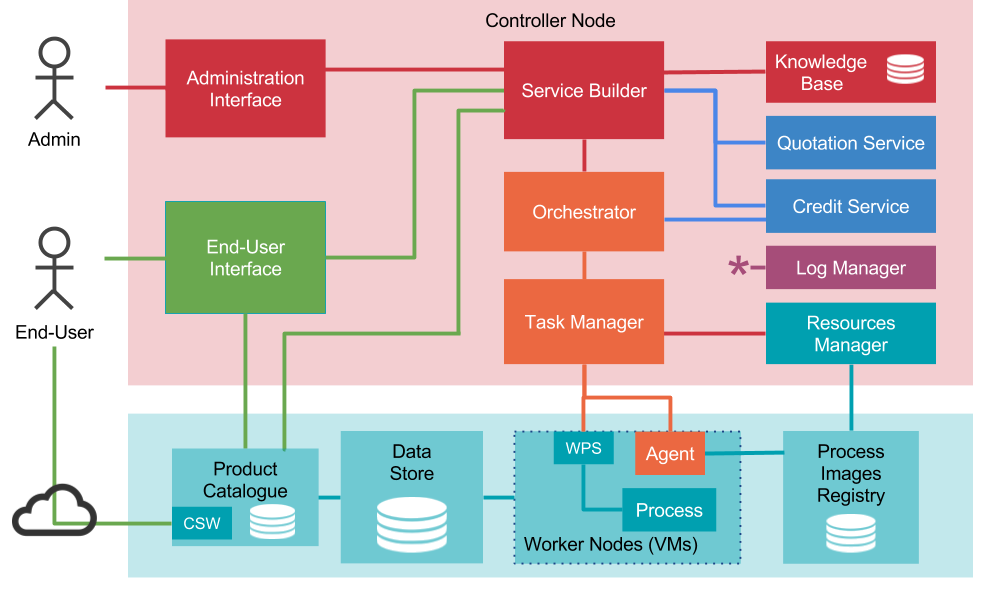
\includegraphics[scale=0.4]{img/asb-services}
%    \end{block}
%\end{frame}

\begin{frame}{Automated Service Builder}{}
    \begin{block}{}
      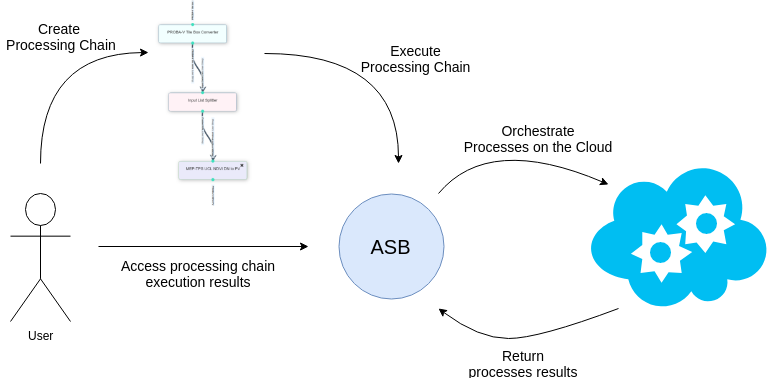
\includegraphics[scale=0.4]{img/asb-user-processingchain}
    \end{block}
\end{frame}



\begin{frame}{Internship content}{Pedagogical content}
    \begin{block}{Development}
      \begin{itemize}
        \item Web applications: Python, Django, Go, Javascript
        \item Git, Gitlab, JIRA
        \item Container technologies
      \end{itemize}
    \end{block}
    \begin{block}{System administration}
      \begin{itemize}
        \item Linux systems
        \item Shell scripting
        \item Network setup and administration
        \item Cloud infrastructure (using Mesos/Marathon)
      \end{itemize}
    \end{block}
\end{frame}

\begin{frame}{Internship objectives}
    \begin{block}{Development}
      \begin{itemize}
        \item Single Sign-On: Centralized login and user informations
        \item Common library to share between components
        \item Improve deployment of the platform
        \item Provide a way to customize the platform by means of project \textit{plugins}
      \end{itemize}
    \end{block}
    \begin{block}{System administration}
      \begin{itemize}
        \item Deploy operational platform for customers
        \item Maintain the cloud environment used by the platform
      \end{itemize}
    \end{block}
\end{frame}

%\begin{frame}{Conclusion}{Results}
%  \begin{block}{Signe Sign-On: by integrating a new core component}
%      \begin{center}
%        \begin{itemize}
%          \item  Without SSO
%          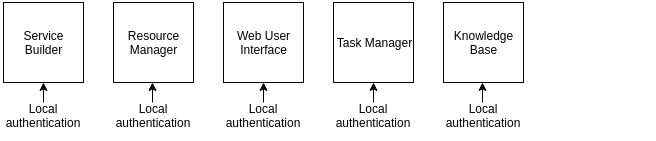
\includegraphics[scale=0.4]{img/asb-sso_off}
%          \item  With SSO
%          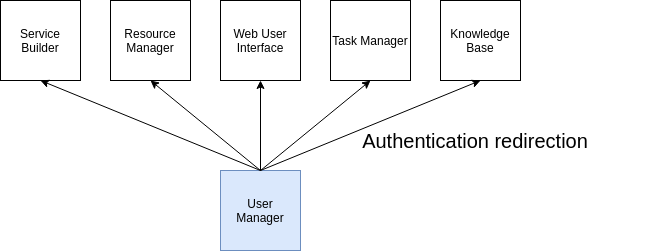
\includegraphics[scale=0.4]{img/asb-sso}
%      \end{itemize}
%      \end{center}
%  \end{block}
%\end{frame}

\begin{frame}{Objectives results}
  \begin{block}{Single Sign-On}
  \begin{itemize}
    \item Implemented by extending the platform with a new service
  \end{itemize}
  \end{block}
  \begin{block}{Shared library, assets and plugins}
    \begin{itemize}
      \item Shared library: implemented and integrated in all core components
      \item Implemented in the shared library: configuration module to choose a deployment mode
      \item Implemented in common library: plugin module to customized to component
    \end{itemize}
  \end{block}
  \begin{block}{System administration}
    \begin{itemize}
      \item Operation services are running and available to customers
    \end{itemize}
  \end{block}
\end{frame}


\begin{frame}{Educational skills used}{Technical skills}

\begin{block}{Programming}
  \begin{itemize}
    \item Python, and programming in general, was a big part of the internship
    \item Capability of learning new programming languages (Go, etc)
    \item Frontend development learned during school projects
  \end{itemize}
\end{block}
\begin{block}{System administration}
  \begin{itemize}
    \item \textit{Administration Systéme} and \textit{Réseaux} were very helpful
    \item \textit{Systéme d'exploitation} for bash scripting and OS comprehension
  \end{itemize}
\end{block}
\end{frame}
\begin{frame}{Educational skills used}{Soft skills}

\begin{block}{Useful skills acquired while being a student:}
  \begin{itemize}
    \item Research to solve problems
    \item Writting documentation in English
    \item Reporting problem solutions
  \end{itemize}

\end{block}
\end{frame}

\begin{frame}{What have I learned}
\begin{block}{Time Management}
  \begin{itemize}
    \item Write everyday about the work done, and how many hours
    \item Time tracking allow to make prediction for the future
  \end{itemize}
\begin{block}{Project Management}
  \begin{itemize}
    \item Documentation is a big part of the job
    \item Daily meeting/discussion are important
  \end{itemize}
  \end{block}
\end{block}
\begin{block}{European Projects participation:}
  \begin{itemize}
    \item Worked on European projects with International Consortium
    \item Each partner is responsible for Work-Packages
    \item I participated in a meeting with all partners in Athens
  \end{itemize}
\end{block}

\end{frame}

\begin{frame}{Retrospective}{Management, deadlines and methodology}
\begin{block}{Time management is important:}
  \begin{itemize}
    \item Small team (2 of us) and a lot of projects (4/5)
    \item Deadlines were met, but with overtime..
    \item Predication are hard to make
  \end{itemize}

\end{block}

\begin{center}
  Emphasize the fact that project management and prioritization is very important
\end{center}
\end{frame}

\begin{frame}{Retrospective}{}
\begin{block}{Integration in the company}
  \begin{itemize}
    \item Already worked 2 years as a student for the System Administration team
    \item Easier to integrate in the team and getting worked done
    \item Small team: easier to interact and discuss
  \end{itemize}
\end{block}
\begin{block}{Downside}
  \begin{itemize}
    \item Internship was very technical
    \item I wrote documentation only for the team
    \item No \textit{real} presentation made during the internship
  \end{itemize}
\end{block}
\end{frame}


\begin{frame}{Retrospective}{Perception}
\begin{block}{Computer scientist ?}
  \begin{itemize}
    \item Broad field, with different finalities
    \item Software Engineer, DevOps, Developer, etc: can mean the same thing or
    be completely different depending on the company
    % \item Software Engineering is an interesting position in computer science
    \item Work can be completely different depending on the Team/Project
  \end{itemize}
\end{block}
\begin{block}{Impact on the company}
  \begin{itemize}
    \item Worked on a product that is used for production
    \item Small team, so responsable very fast
    \item Still in the company after the internship, still working on ASB!
  \end{itemize}
\end{block}
\end{frame}


%%%%%%%%%%%%%%%%

%{\aauwavesbg
%\begin{frame}[allowframebreaks]
%    \frametitle{References}
%\bibliographystyle{plain}
%\bibliography{../thesis}
%\end{frame}}

{\aauwavesbg
\begin{frame}[plain,noframenumbering]
  \finalpage{Thank you!}
\end{frame}}

\end{document}
